\documentclass[11pt,a4paper]{article}
\usepackage{fontspec}
\setmainfont{TeX Gyre Pagella}
\newfontfamily\headfont{Inter}[UprightFont=*-ExtraBold,BoldFont=*-ExtraBold,Extension=.otf,Path=/usr/share/fonts/opentype/inter/]
\usepackage[a4paper,margin=2.3cm]{geometry}
\usepackage{graphicx,booktabs,float,caption,array,xcolor}
\usepackage[hidelinks]{hyperref}
\usepackage{titlesec}
\usepackage[round]{natbib}
\usepackage{setspace}
\setstretch{1.05}
\renewcommand{\topfraction}{0.9}
\renewcommand{\bottomfraction}{0.8}
\renewcommand{\textfraction}{0.1}
\renewcommand{\floatpagefraction}{0.75}
\setlength{\parindent}{0pt}
\setlength{\parskip}{0.55em}
\titleformat{\section}{\headfont\Large}{\thesection}{0.8em}{}
\titleformat{\subsection}{\headfont\large}{\thesubsection}{0.8em}{}
\captionsetup{font=small,labelfont=bf}
\urlstyle{same}
\hypersetup{pdftitle={Who Was Big When? League Position and Crowds of Every English League Club},pdfauthor={Tristan Hotham}}

\begin{document}
\begin{center}
{\Large\bfseries Who Was Big When?\par}
\vspace{0.4em}
{\large League position and crowds of every English league club,\\1888-89 to 2024-25\par}
\vspace{1.2em}
{\large Tristan Hotham\par}
\vspace{0.3em}
{\small Independent researcher\\
ORCID: 0000-0003-4931-9349\\
DOI: \href{https://doi.org/10.5281/zenodo.23844507}{https://doi.org/10.5281/zenodo.23844507}\par}
\vspace{0.8em}
2026
\end{center}

\begin{quote}
\small
\begin{center}\textbf{Abstract}\end{center}
I rebuild the final table of every Football League and Premier League season from 1888-89 to 2024-25 (126 seasons, 210,019 matches, 147 clubs) and join each club's average home league crowd for every season it is recorded, to map where English league football has been big and when. Total league crowds rose from about 635 thousand in the first season to a peak of 41.2 million in 1948-49, fell in 27 of the next 37 seasons to 16.5 million in 1985-86 (60\% below the peak), and recovered to 36.4 million in 2024-25. The geography moved south. Before 1915 the North held 62\% of top-flight places and London and the South 6\%; since 2010 the shares are 36\% and 43\%, and the crowd-weighted centre of the top flight has moved about 78 km south. Titles stayed northern (87 of 126), concentrated since 2000 in Manchester and Liverpool. 39 of the 113 towns that have had a league club have none today. Every club's peak, by league position and crowd, is listed in the accompanying data.

\textbf{Keywords:} football; English Football League; Premier League; attendance; sports history; regional geography; North and South; mapping
\end{quote}

\section{Introduction}
The Football League began in September 1888 with twelve clubs, six from Lancashire and six from the Midlands. It had no club from London until 1893-94 and no champion from London until 1930-31. In 2024-25 seven of the twenty Premier League clubs were from London. Between those two points English football went through its great expansion before the First World War, a second expansion into four divisions after it, an extraordinary peak of attendance after the Second World War, a long decline to the mid 1980s and a recovery that the Premier League era has made top-heavy in money if not in crowds \citep{russell,dobson,szymanski}.

Histories of the game describe these changes well, but usually club by club or through national totals. This paper puts them on one map. For every season since 1888 I rebuild the final tables from match results, place every club at its ground and size it by its average home league crowd. The aim is descriptive: to show, with numbers, who was big when and where. An interactive version, with a season slider, play button, club search and a sparkline for every club, is at \url{https://maps.tristanhotham.com/who-was-big-when/}.

\section{Data}
\textbf{Match results.} James Curley's engsoccerdata package \citep{curley} holds every English league match in the top four tiers from 1888-89, with date, teams, score, division and tier. The 2022-23 season is missing from the version used here, so its 2,036 regular-season matches were taken from the openfootball project \citep{openfootball} and their club names matched to engsoccerdata's. Play-off matches are not included. In all, 210,019 matches over 126 seasons; the league did not play during the two world wars, and the abandoned 1939-40 season is left out.

\textbf{Crowds.} Average home league gates per club and season were taken from englishfootballleaguetables.co.uk \citep{eflt}, which compiles them from official returns and, for early seasons, contemporary reports. Its first table each season gives every club's division, average home league gate and average away gate. I matched its club names to engsoccerdata's within each season: exact names, then normalised names, then a short list of historical names (Small Heath, Newton Heath, Ardwick, The Wednesday, Woolwich Arsenal and others), then a unique match on the first word. 5 names could not be matched, all of them clubs whose records were expunged (Leeds City 1919-20, Wigan Borough 1931-32, Accrington Stanley 1961-62, Aldershot 1991-92, Maidstone United 1992-93). Football Alliance clubs in the source's early tables were left out. There are no figures for 2020-21, played behind closed doors, and the source page saved for 2021-22 was a copy of 2022-23, so 2021-22 has no crowd data here. The 2024-25 figures are the last complete season. In all 9,644 club-seasons have a crowd.

\textbf{Places.} Each club is placed at its present or last ground from engsoccerdata's club table, corrected for two clubs, and assigned the ONS region, ceremonial county and nation that point falls in \citep{ons}. For the North and South comparison regions are grouped into five areas: the North (North East, North West, Yorkshire and the Humber), the Midlands (East and West Midlands), London, the rest of the South (East, South East, South West) and Wales. Each club is also given by hand the town it stands for; the London clubs share one town, London.

\section{Methods}
\textbf{Tables.} Each season and division's table was computed from the matches: two points for a win until 1980-81 and three from 1981-82; ties broken by goal average (goals scored divided by goals conceded) until 1975-76 and by goal difference from 1976-77 (the top flight of 1975-76 already on goal difference, as in engsoccerdata's own table function), then goals scored. Points deductions were applied from engsoccerdata's list to 2014-15 and from published tables after that (for example Derby County, minus 21 in 2021-22, and Everton, minus 8 in 2023-24). The third and fourth tiers of 2019-20, ended early, were ranked by points per game. Matches of clubs whose records were expunged were removed, and Leeds City's matches of 1919-20 were credited to Port Vale, who took over their fixtures. The rebuilt champions and some final places were checked against the known record in more than fifty seasons.

\textbf{League position.} To compare clubs across divisions each club gets a pyramid rank: the number of clubs in higher tiers plus its position in its division. The champion is 1 and, from 1950-51, the bottom club of the fourth tier is 92. The two regional third divisions of 1921-22 to 1957-58 share the same offset.

\textbf{Crowds.} A club's league crowd for a season is its average home league gate times its number of home league matches; the season total is the sum over clubs. Cup, play-off and European matches are not counted. Area shares of top-flight places are shares of club-seasons; area shares of crowds are shares of these totals. The crowd-weighted centre of the top flight is the mean latitude and longitude of top-flight grounds weighted by home average.

\textbf{Lost towns and peaks.} A town lost league football if it had a league club in some season and none in 2025-26 (the 2024-25 clubs, less the two relegated from League Two and plus the two promoted from the National League at the end of that season). A club's best decade is the decade in which its average pyramid rank was best, counting only decades with at least three of its seasons.

\section{Results}
\subsection{The map through time}
Figure~\ref{fig:maps} shows five seasons. In 1888-89 the league was a band from Preston to Birmingham. By 1913-14 it had 40 clubs, with the North East, Yorkshire and London added. By 1948-49 the 88 clubs filled England and South Wales, and the big circles were in the industrial North and Midlands as well as London. In 1985-86 every circle had shrunk. In 2024-25 the biggest circles are in London, Manchester, Liverpool, Newcastle and Birmingham, and the lower divisions are spread more evenly across the South.

\begin{figure}[tbp]\centering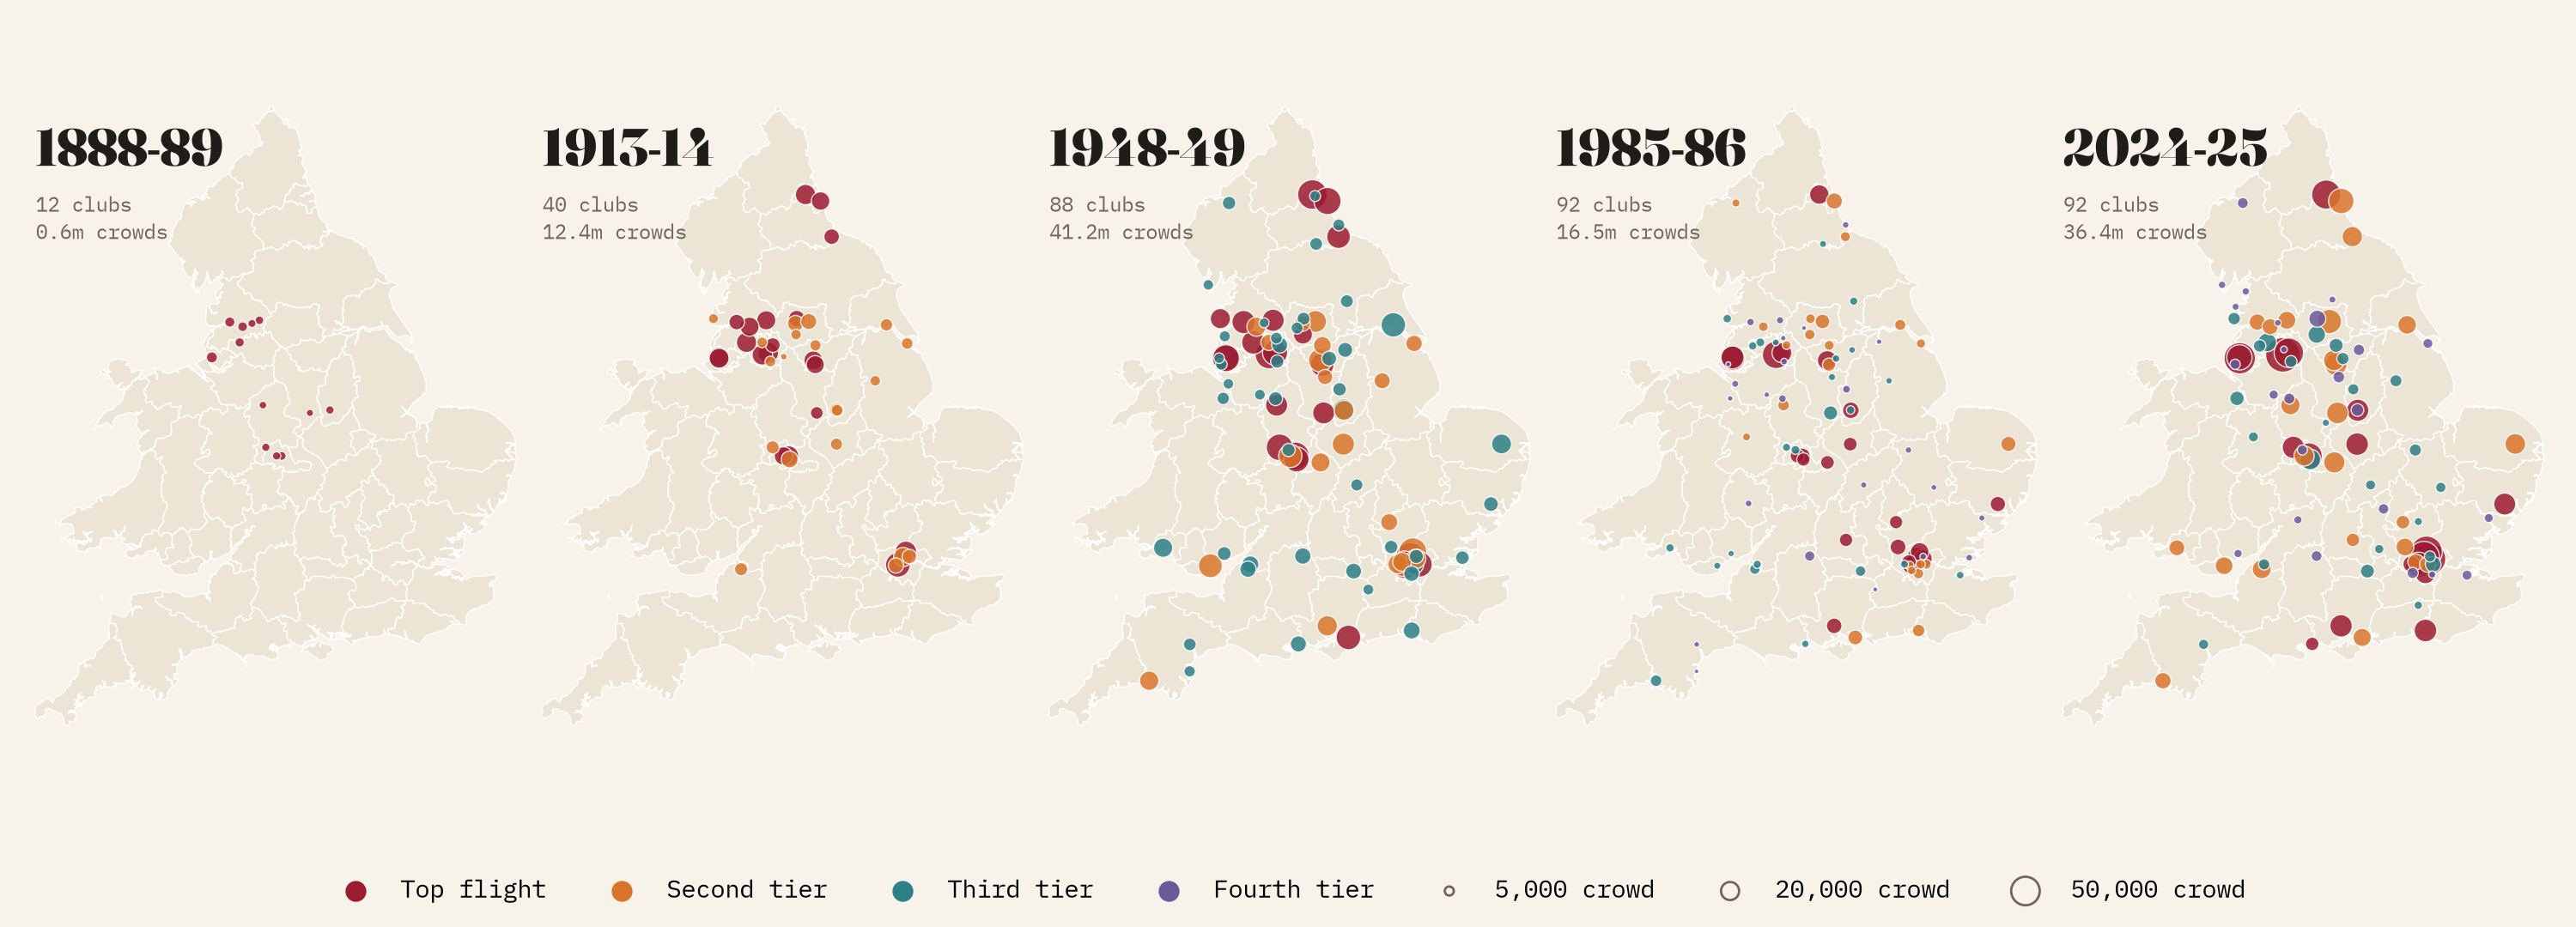
\includegraphics[width=\textwidth]{f_maps.png}
\caption{Every league club in five seasons, at its present or last ground. Circle area: average home league crowd. Colour: tier.}\label{fig:maps}\end{figure}

\subsection{Crowds}
Total league crowds (Figure~\ref{fig:crowds}) grew almost every season before the First World War, from about 635 thousand in 1888-89 to 12.4 million in 1913-14. Between the wars they peaked at 27.9 million in 1937-38. After the Second World War they reached 41.2 million in 1948-49, an average of 22,318 a match across all four divisions and 38,766 in the top flight. Crowds then fell in 27 of 37 seasons, to 16.5 million in 1985-86, when the top-flight average was 19,581. The recovery started in 1986-87, before the Taylor Report \citep{taylor} and the all-seater grounds it led to, and before the Premier League. By 2024-25 the total was 36.4 million, 88\% of the peak; only 6 seasons, 1947-48 to 1952-53, had more.

The top-flight average rose from 21,136 in 1992-93 to 40,430 in 2024-25, a factor of 1.9. Yet the top flight's share of all league spectators was 42\% in 2024-25, against 43\% in 1948-49. The lower three divisions drew 21.1 million, against 23.3 million at the peak. Table~\ref{tab:crowds} gives the milestones.

\begin{figure}[tbp]\centering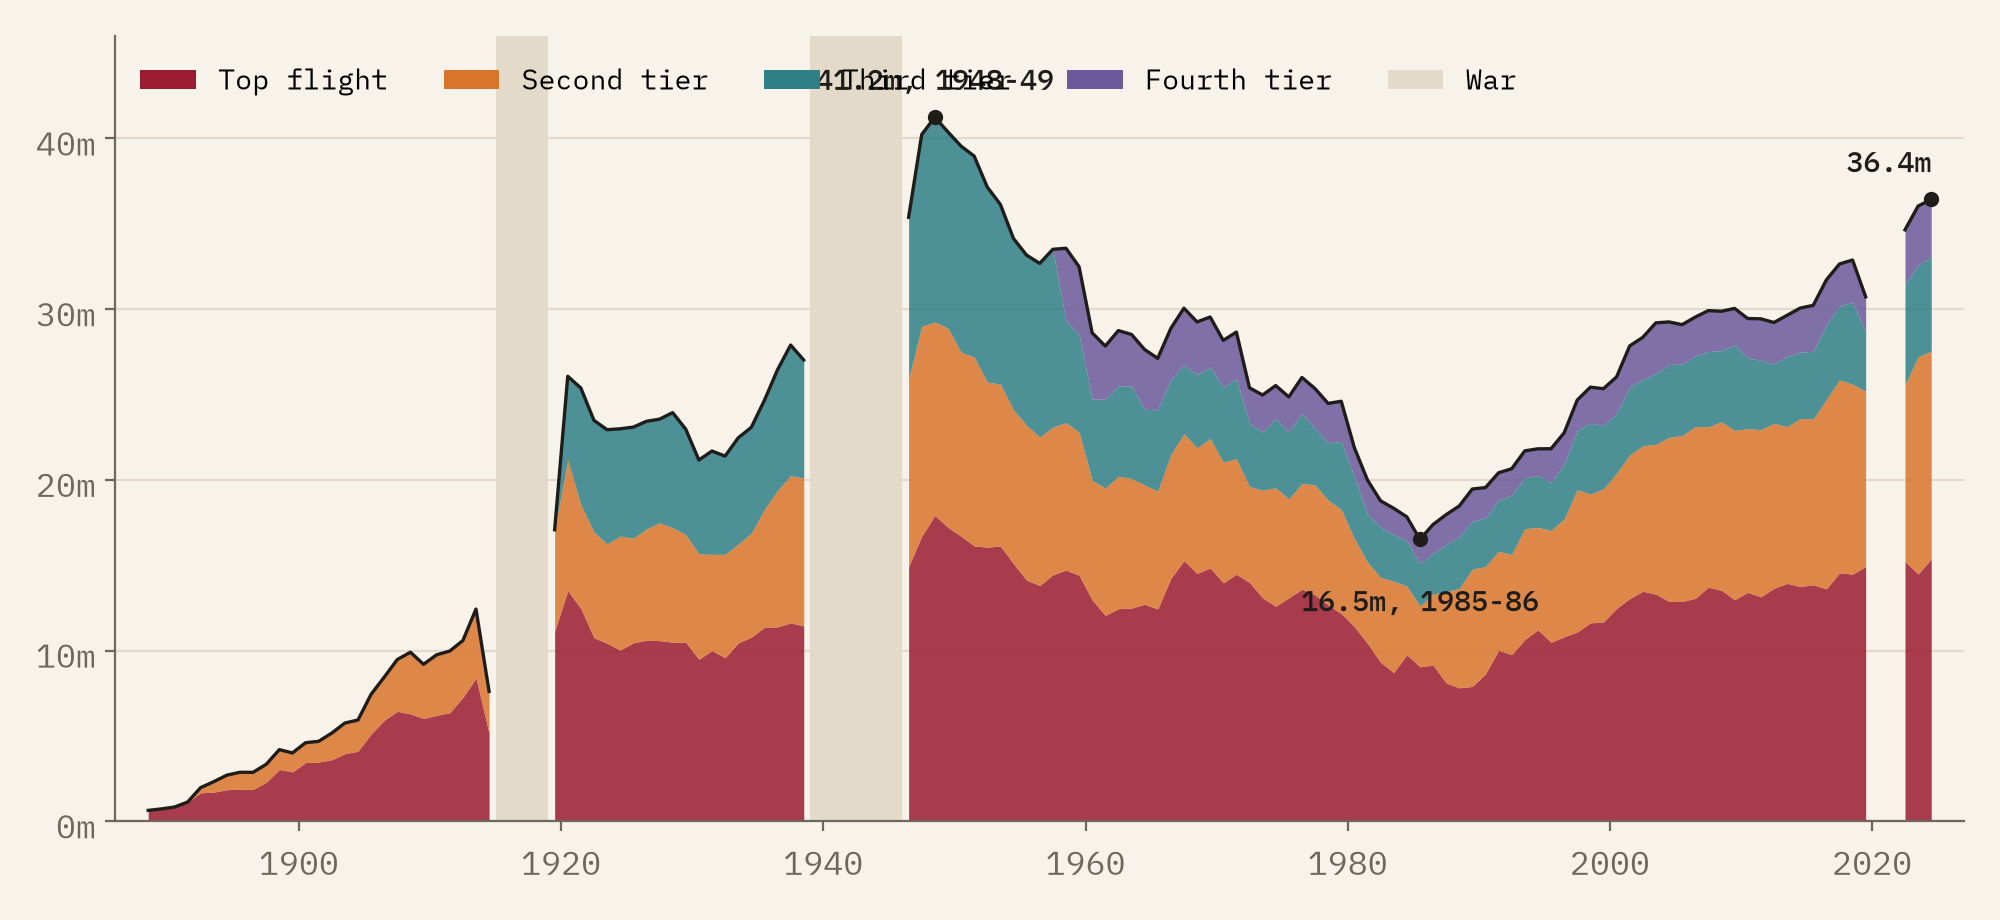
\includegraphics[width=.95\textwidth]{f_crowds.png}
\caption{Total league crowd each season, stacked by tier: average home league gate times home league matches. Shaded: the wars. No data for 2020-21 and 2021-22.}\label{fig:crowds}\end{figure}

\begin{table}[tbp]\centering\small\caption{Crowd milestones. Total: millions at league matches; averages per match.}\label{tab:crowds}\begin{tabular}{llrrrr}\toprule Season & & Clubs & Total (m) & Average & Top flight\\\midrule
1888-89 & First season & 12 & 0.6 & 4,812 & 4,812\\
1913-14 & Last before the First World War & 40 & 12.4 & 16,353 & 22,067\\
1937-38 & Inter-war peak & 88 & 27.9 & 15,095 & 25,144\\
1948-49 & All-time peak & 88 & 41.2 & 22,318 & 38,766\\
1966-67 & England's World Cup season & 92 & 28.9 & 14,236 & 30,777\\
1985-86 & Low point & 92 & 16.5 & 8,140 & 19,581\\
1992-93 & First Premier League season & 92 & 20.6 & 10,182 & 21,136\\
2024-25 & Latest complete season & 92 & 36.4 & 17,892 & 40,430\\
\bottomrule\end{tabular}\end{table}

\subsection{North and South}
In the league's first era, to 1915, the North held 62\% of top-flight places, the Midlands 32\% and London and the rest of the South 6\% (Figure~\ref{fig:balance}, Table~\ref{tab:eras}). The North won 21 of the 27 titles before 1915 and the Midlands the rest. London's first top-flight club arrived in 1904-05; London had 3 top-flight clubs in 1930-31 and a maximum of 8, in 1989-90. From 2010 the North's share of top-flight places was 36\% and the South's, London included, 43\%; in 2024-25 the Premier League had 7 London clubs, 4 from the rest of the South, 4 from the Midlands and 5 from the North. Crowds moved less: the North's share of all league crowds fell from 60\% to 40\%, and the South's rose from 13\% to 39\%. Weighted by crowds, the centre of the top flight moved about 78 km south, from near Chapel-en-le-Frith on the edge of the Peak District to near Market Bosworth in Leicestershire.

Titles stayed northern. Of 126 champions, 87 were from the North, 21 from London, 15 from the Midlands and 3 from the rest of the South (Portsmouth first, in 1948-49); no Welsh club has won the English title. Since 2000-01 the North has won 17 of 25, all of them for clubs from Manchester or Liverpool. What the North lost was not its great city clubs but the depth of its towns.

\begin{figure}[tbp]\centering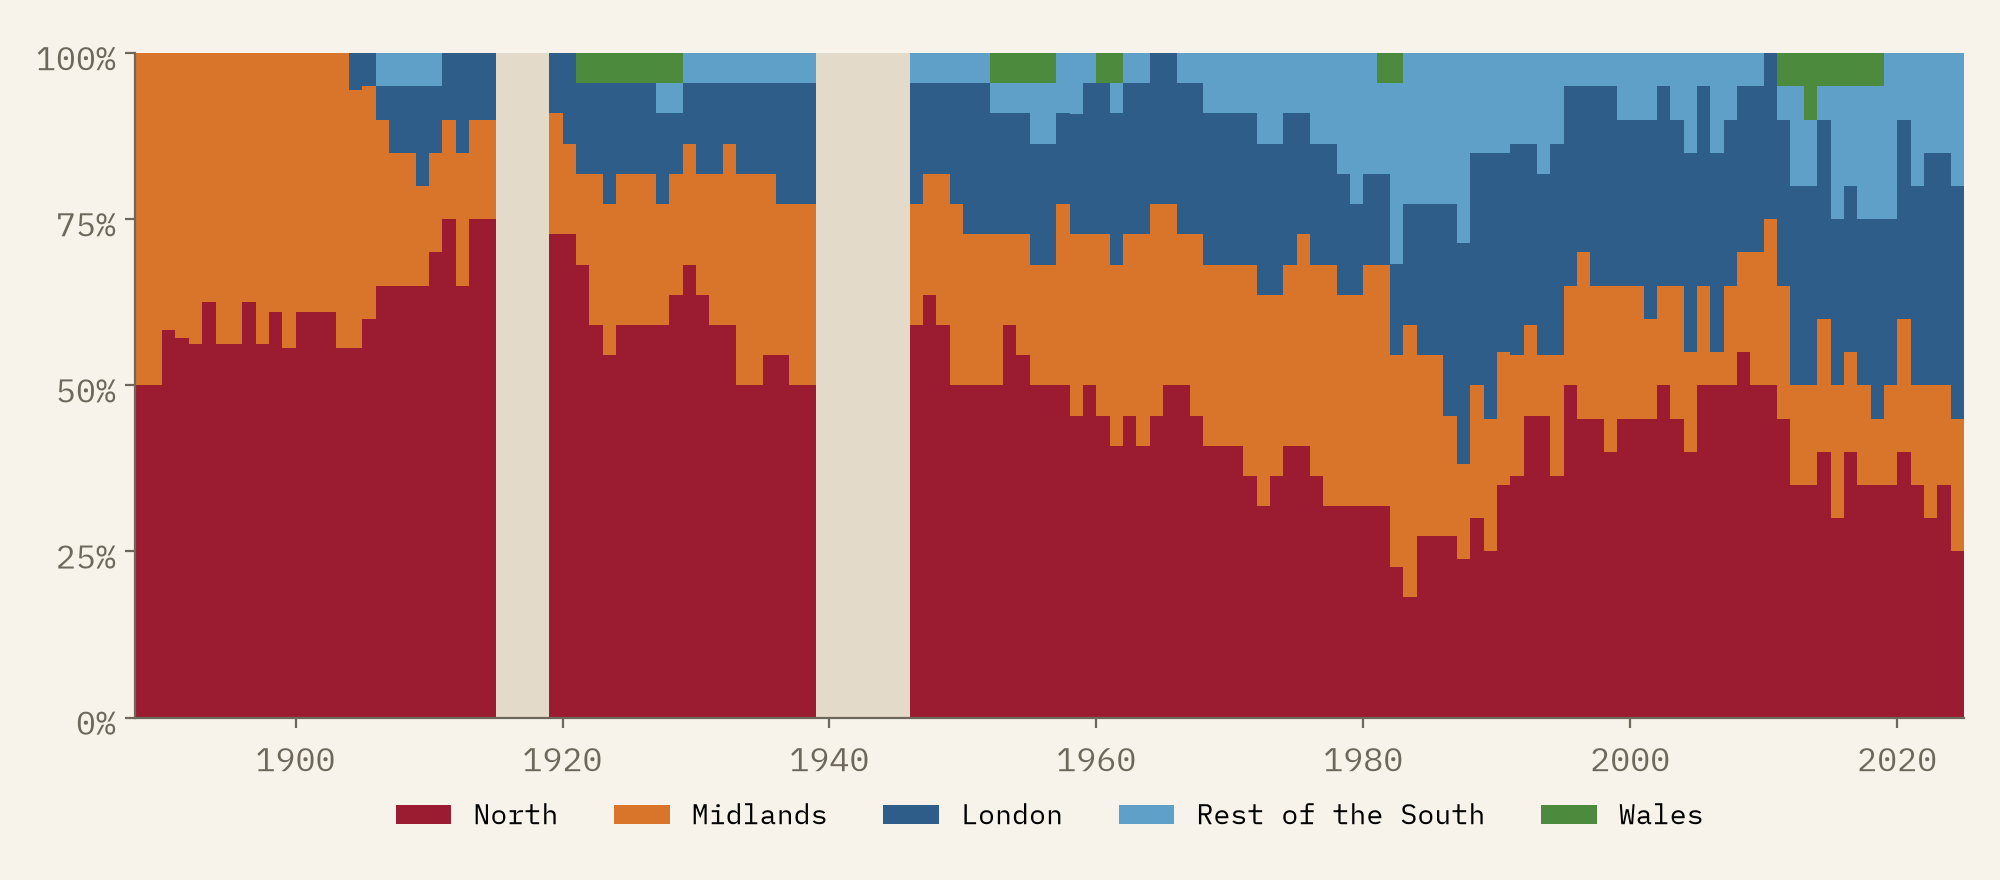
\includegraphics[width=.95\textwidth]{f_balance.png}
\caption{Share of top-flight clubs each season by area. Shaded: the wars.}\label{fig:balance}\end{figure}

\begin{table}[tbp]\centering\footnotesize\setlength{\tabcolsep}{3.5pt}\caption{Area shares by era, per cent: top-flight places (N North, M Midlands, L London, S rest of the South, W Wales), all league crowds, and titles (North/Midlands/London/South).}\label{tab:eras}\begin{tabular}{lrrrrrrrrrr}\toprule & \multicolumn{5}{c}{Top-flight places} & \multicolumn{4}{c}{Crowds} & Titles\\ Era & N & M & L & S & W & N & M & L & S & N/M/L/S\\\midrule
1888 to 1915 & 62 & 32 & 4 & 1 & 0 & 60 & 27 & 11 & 2 & 21/6/0/0\\
1919 to 1939 & 59 & 22 & 14 & 3 & 2 & 45 & 20 & 19 & 12 & 14/1/5/0\\
1946 to 1967 & 50 & 24 & 20 & 5 & 2 & 44 & 20 & 17 & 16 & 10/3/5/3\\
1967 to 1992 & 33 & 28 & 23 & 16 & 0 & 40 & 21 & 17 & 19 & 18/4/3/0\\
1992 to 2010 & 46 & 17 & 28 & 9 & 0 & 43 & 20 & 18 & 17 & 12/0/6/0\\
2010 to 2025 & 36 & 17 & 29 & 14 & 3 & 40 & 18 & 19 & 19 & 12/1/2/0\\
\bottomrule\end{tabular}\end{table}

\subsection{The best-supported club}
The club with the biggest average home crowd each season (Figure~\ref{fig:kings}) was Everton for the league's first decade, then Aston Villa, then Newcastle United and Chelsea in turn before the First World War, and Arsenal through the 1930s. After the Second World War it passed between Newcastle, Tottenham, Arsenal, Chelsea, Everton, Liverpool and Manchester United, and every recorded season since 1993-94 it has been Manchester United, who have led in 56 seasons in all. The biggest average in the data is 75,826, at Old Trafford in 2006-07. 9 different clubs have had the biggest crowd in at least one season.

\begin{figure}[tbp]\centering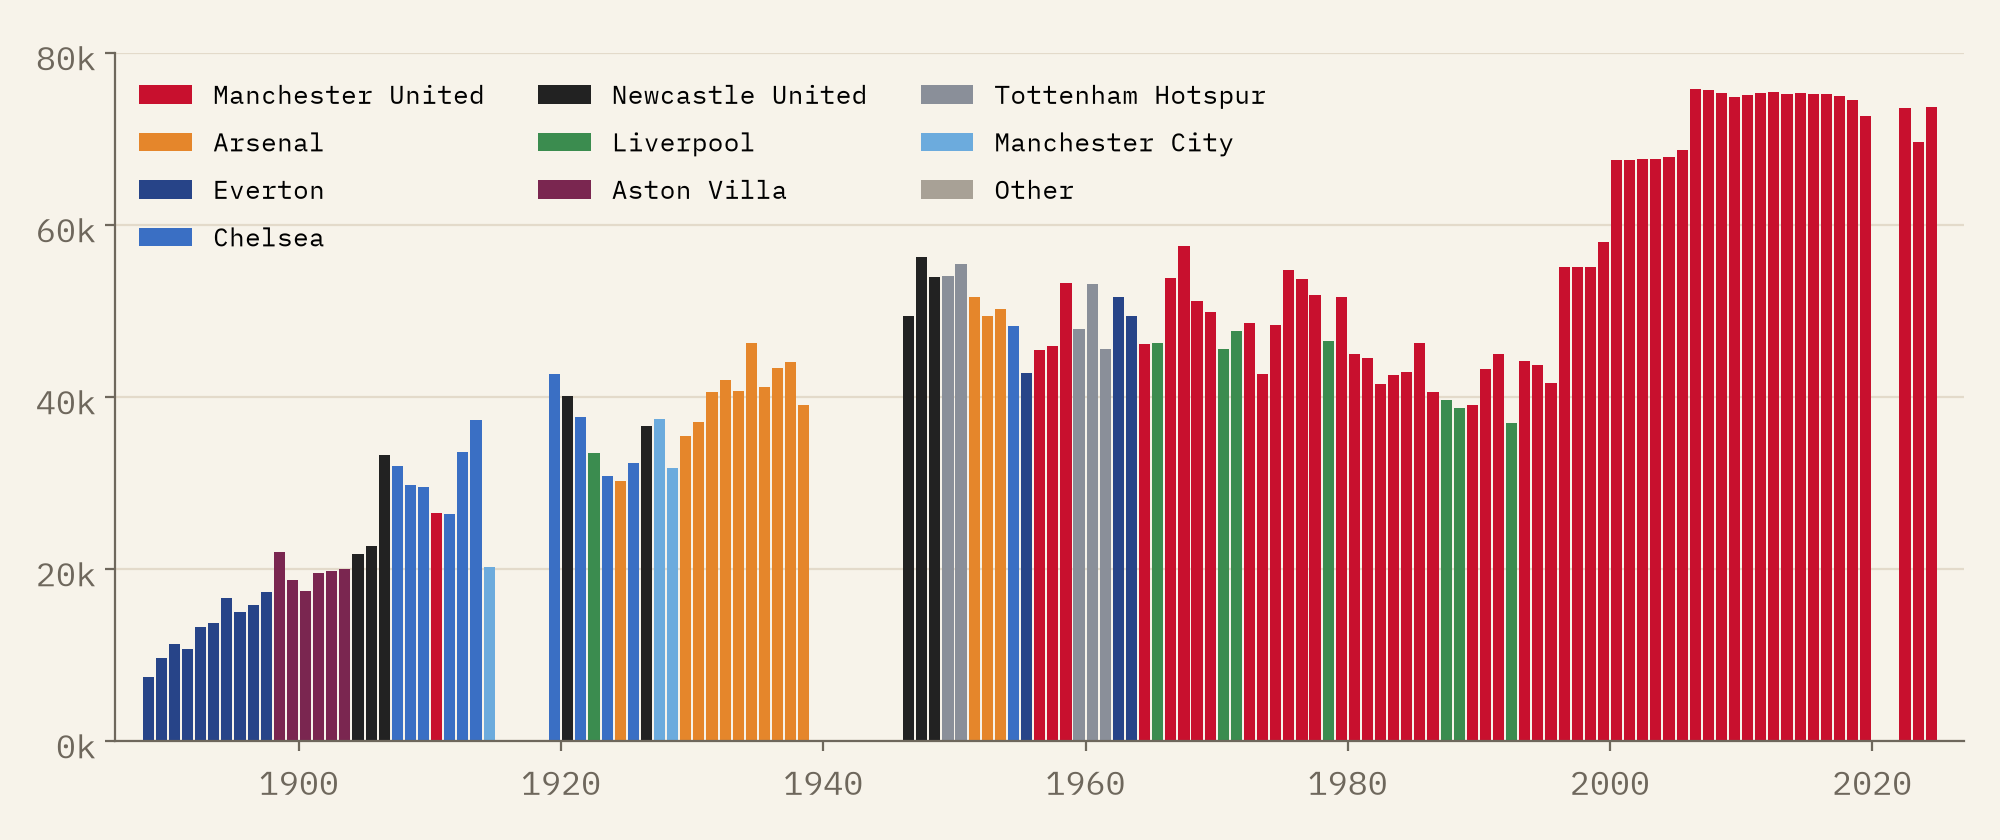
\includegraphics[width=.95\textwidth]{f_kings.png}
\caption{Highest average home league crowd each season, coloured by club.}\label{fig:kings}\end{figure}

\subsection{Towns that lost league football}
113 towns and cities have had a league club; 74 have one in 2025-26. The other 39 (Figure~\ref{fig:lost}, Table~\ref{tab:lost}) fall into three groups. The first left before the First World War: small Lancashire and Cheshire towns such as Darwen, Bootle and Northwich, and Glossop, the smallest town to have had a top-flight club (1899-00). The second left between the wars, many of them from the regional third divisions: Merthyr Tydfil, Aberdare, Ashington, Durham, Nelson, Stalybridge, South Shields. The third, 20 towns, have lost their club since 2000, through relegation to the National League or, for Bury in 2019, expulsion after 114 seasons. 4 lost towns once had a top-flight club: Bury, Darwen, Carlisle and Glossop. Carlisle and Morecambe left at the end of 2024-25; Barnet and Oldham, promoted back into the league for 2025-26, are not counted. Five clubs came back after ten or more seasons away: Barrow (48 seasons out), Newport County, Aldershot (as a refounded club), Wrexham and Stockport County.

\begin{figure}[tbp]\centering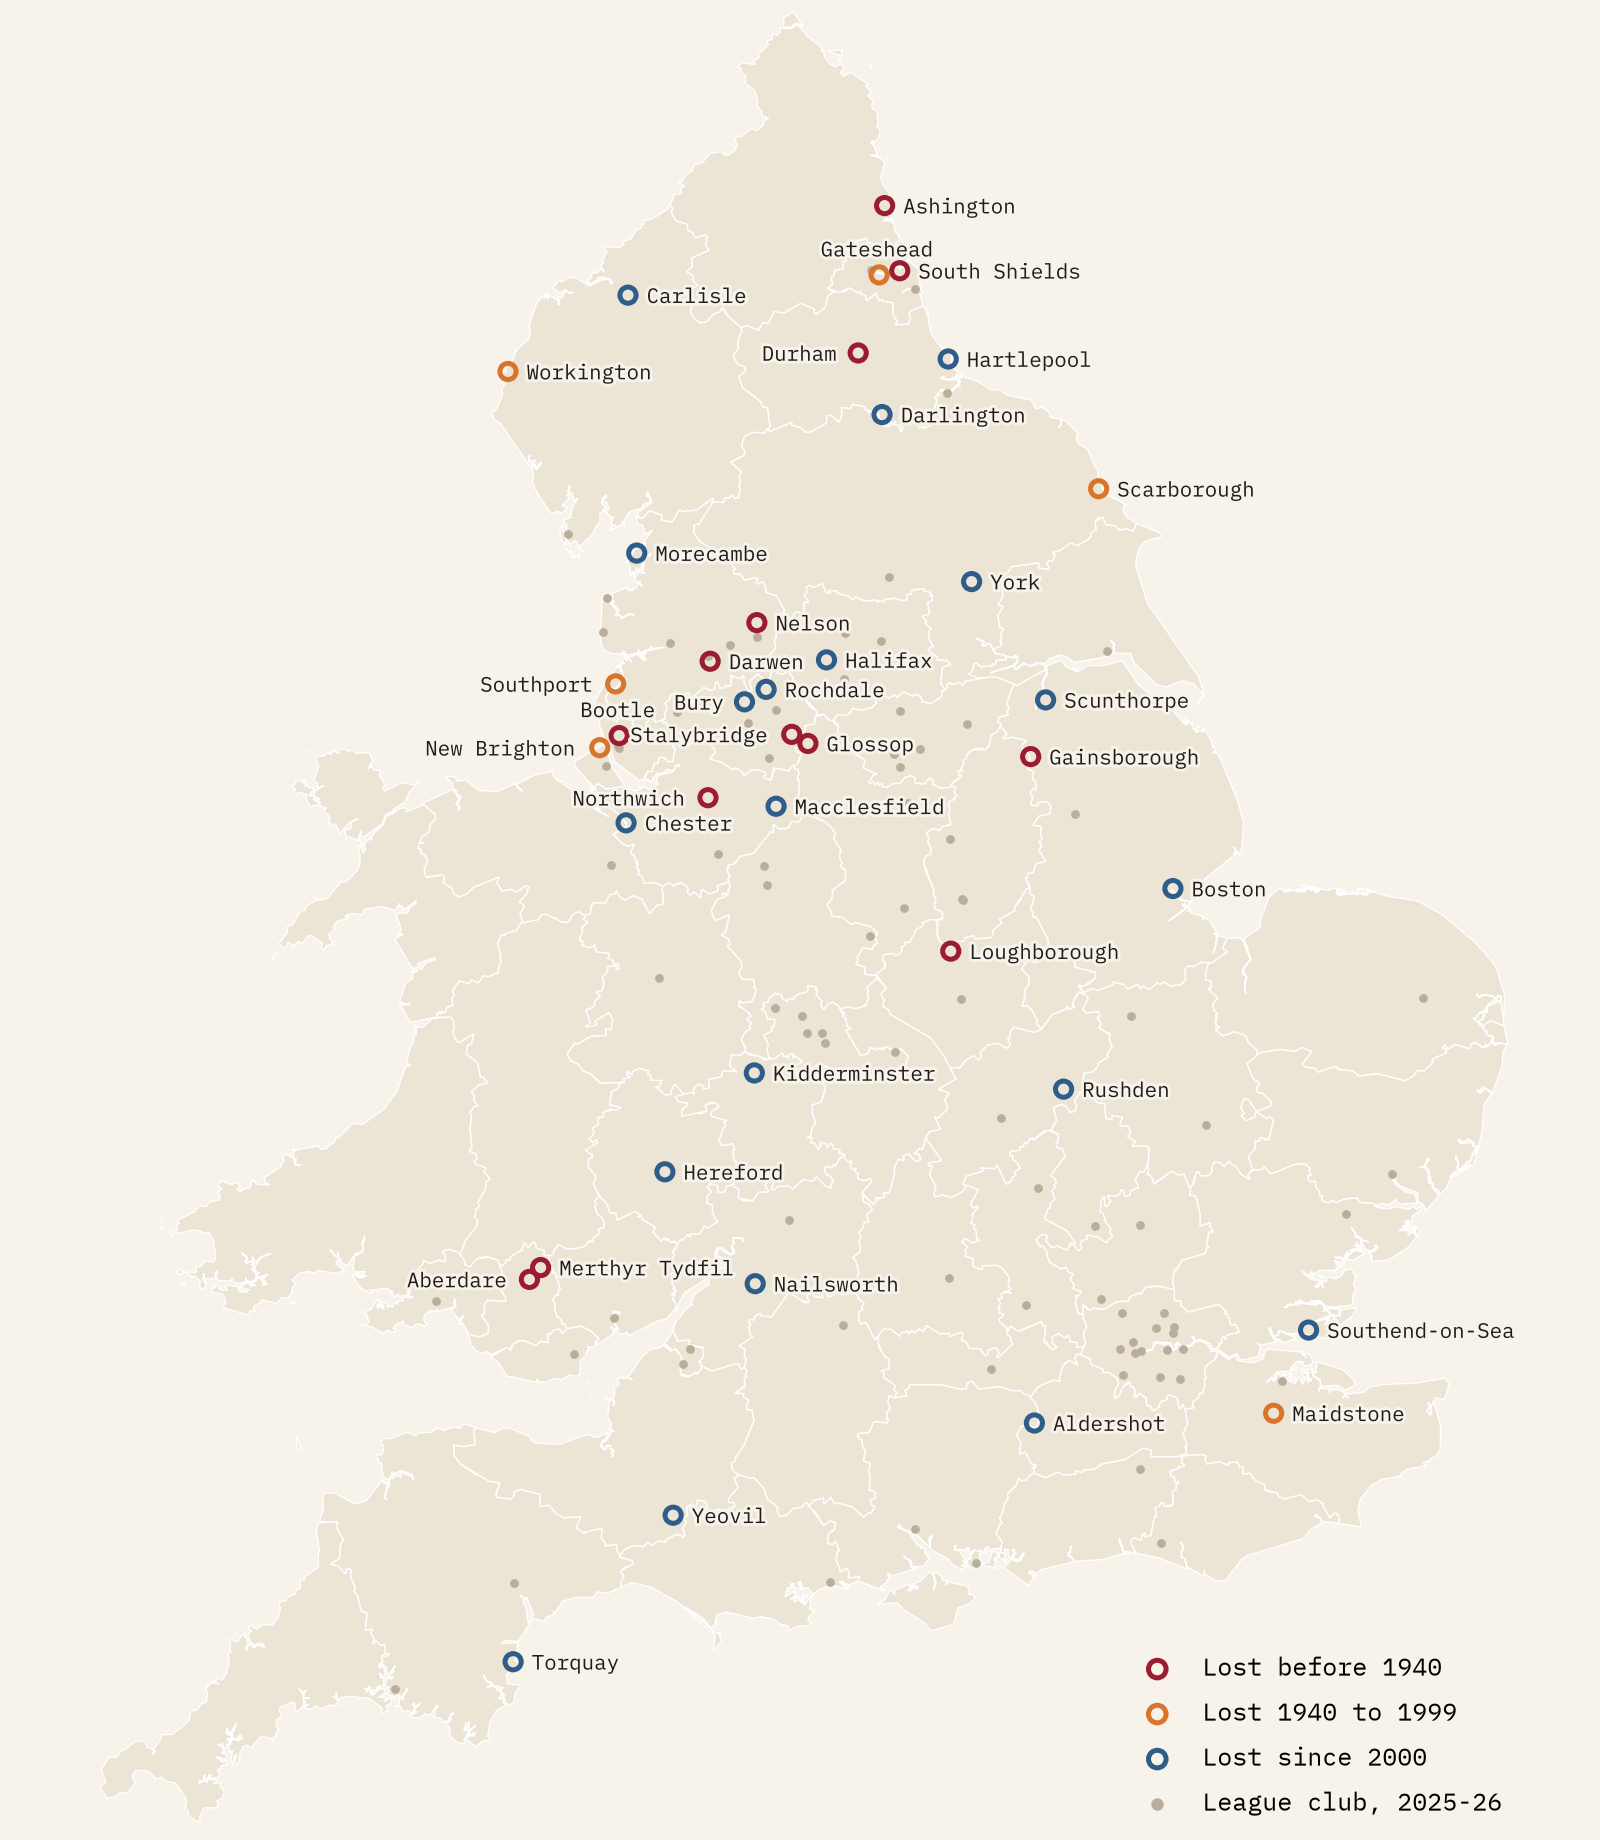
\includegraphics[width=.72\textwidth]{f_lost.png}
\caption{The 39 towns with a league club in some season and none in 2025-26, by when they lost it. Grey: league clubs in 2025-26.}\label{fig:lost}\end{figure}

\begin{table}[tbp]\centering\scriptsize\caption{The 39 towns that had a league club and have none in 2025-26, most recent first. Best: highest finish.}\label{tab:lost}\begin{tabular}{llrll}\toprule Town & Club(s) & Seasons & Last & Best\\\midrule
Carlisle & Carlisle United & 89 & 2024-25 & 22, top tier (1974-75)\\
Morecambe & Morecambe & 18 & 2024-25 & 19, 3rd tier (2021-22)\\
Nailsworth & Forest Green Rovers & 7 & 2023-24 & 24, 3rd tier (2022-23)\\
Hartlepool & Hartlepool United & 91 & 2022-23 & 2, 3rd tier (1956-57)\\
Rochdale & Rochdale & 95 & 2022-23 & 2, 3rd tier (1923-24)\\
Scunthorpe & Scunthorpe United & 72 & 2021-22 & 4, 2nd tier (1961-62)\\
Southend-on-Sea & Southend United & 94 & 2020-21 & 12, 2nd tier (1991-92)\\
Macclesfield & Macclesfield Town & 17 & 2019-20 & 24, 3rd tier (1998-99)\\
Bury & Bury & 114 & 2018-19 & 4, top tier (1925-26)\\
Yeovil & Yeovil Town & 16 & 2018-19 & 24, 2nd tier (2013-14)\\
York & York City & 72 & 2015-16 & 15, 2nd tier (1974-75)\\
Torquay & Torquay United & 78 & 2013-14 & 2, 3rd tier (1956-57)\\
Aldershot & Aldershot & 57 & 2012-13 & 8, 3rd tier (1973-74)\\
Hereford & Hereford United & 31 & 2011-12 & 22, 2nd tier (1976-77)\\
Darlington & Darlington & 81 & 2009-10 & 15, 2nd tier (1925-26)\\
Chester & Chester City & 67 & 2008-09 & 2, 3rd tier (1935-36)\\
Boston & Boston United & 5 & 2006-07 & 11, 4th tier (2003-04)\\
Rushden & Rushden \& Diamonds & 5 & 2005-06 & 22, 3rd tier (2003-04)\\
Kidderminster & Kidderminster Harriers & 5 & 2004-05 & 10, 4th tier (2001-02)\\
Halifax & Halifax Town & 69 & 2001-02 & 2, 3rd tier (1934-35)\\
Scarborough & Scarborough & 12 & 1998-99 & 5, 4th tier (1988-89)\\
Maidstone & Maidstone United & 3 & 1991-92 & 5, 4th tier (1989-90)\\
Southport & Southport & 50 & 1977-78 & 4, 3rd tier (1924-25)\\
Workington & Workington & 26 & 1976-77 & 4, 3rd tier (1956-57)\\
Gateshead & Gateshead & 23 & 1959-60 & 2, 3rd tier (1931-32)\\
New Brighton & New Brighton / New Brighton Tower & 24 & 1950-51 & 4, 2nd tier (1900-01)\\
Nelson & Nelson & 10 & 1930-31 & 21, 2nd tier (1923-24)\\
Merthyr Tydfil & Merthyr Town & 10 & 1929-30 & 8, 3rd tier (1920-21)\\
South Shields & South Shields & 11 & 1929-30 & 6, 2nd tier (1921-22)\\
Ashington & Ashington & 8 & 1928-29 & 8, 3rd tier (1923-24)\\
Durham & Durham City & 7 & 1927-28 & 11, 3rd tier (1921-22)\\
Aberdare & Aberdare Athletic & 6 & 1926-27 & 8, 3rd tier (1921-22)\\
Stalybridge & Stalybridge Celtic & 2 & 1922-23 & 7, 3rd tier (1921-22)\\
Glossop & Glossop North End & 17 & 1914-15 & 18, top tier (1899-00)\\
Gainsborough & Gainsborough Trinity & 16 & 1911-12 & 7, 2nd tier (1896-97)\\
Loughborough & Loughborough & 5 & 1899-00 & 12, 2nd tier (1895-96)\\
Darwen & Darwen & 8 & 1898-99 & 14, top tier (1891-92)\\
Northwich & Northwich Victoria & 2 & 1893-94 & 7, 2nd tier (1892-93)\\
Bootle & Bootle & 1 & 1892-93 & 8, 2nd tier (1892-93)\\
\bottomrule\end{tabular}\end{table}

\subsection{Peaks}
Clubs' best decades are spread across the whole history (Figure~\ref{fig:peaks}). Of the 103 clubs with at least twenty league seasons, 10 had their best decade in the 1890s and 10 are in it now. Preston's best season was the first, the unbeaten double of 1888-89; Huddersfield Town won three titles in a row in the 1920s; Portsmouth won two in a row after the Second World War; and Nottingham Forest went from 3rd in the second tier in 1976-77 to champions in 1977-78. Brighton and Bournemouth, each in the league since the 1920s, had their best seasons in the last decade. The full list, with each club's best finish, best decade and biggest crowd, is in \texttt{data/club\_peaks.csv}.

\begin{figure}[tbp]\centering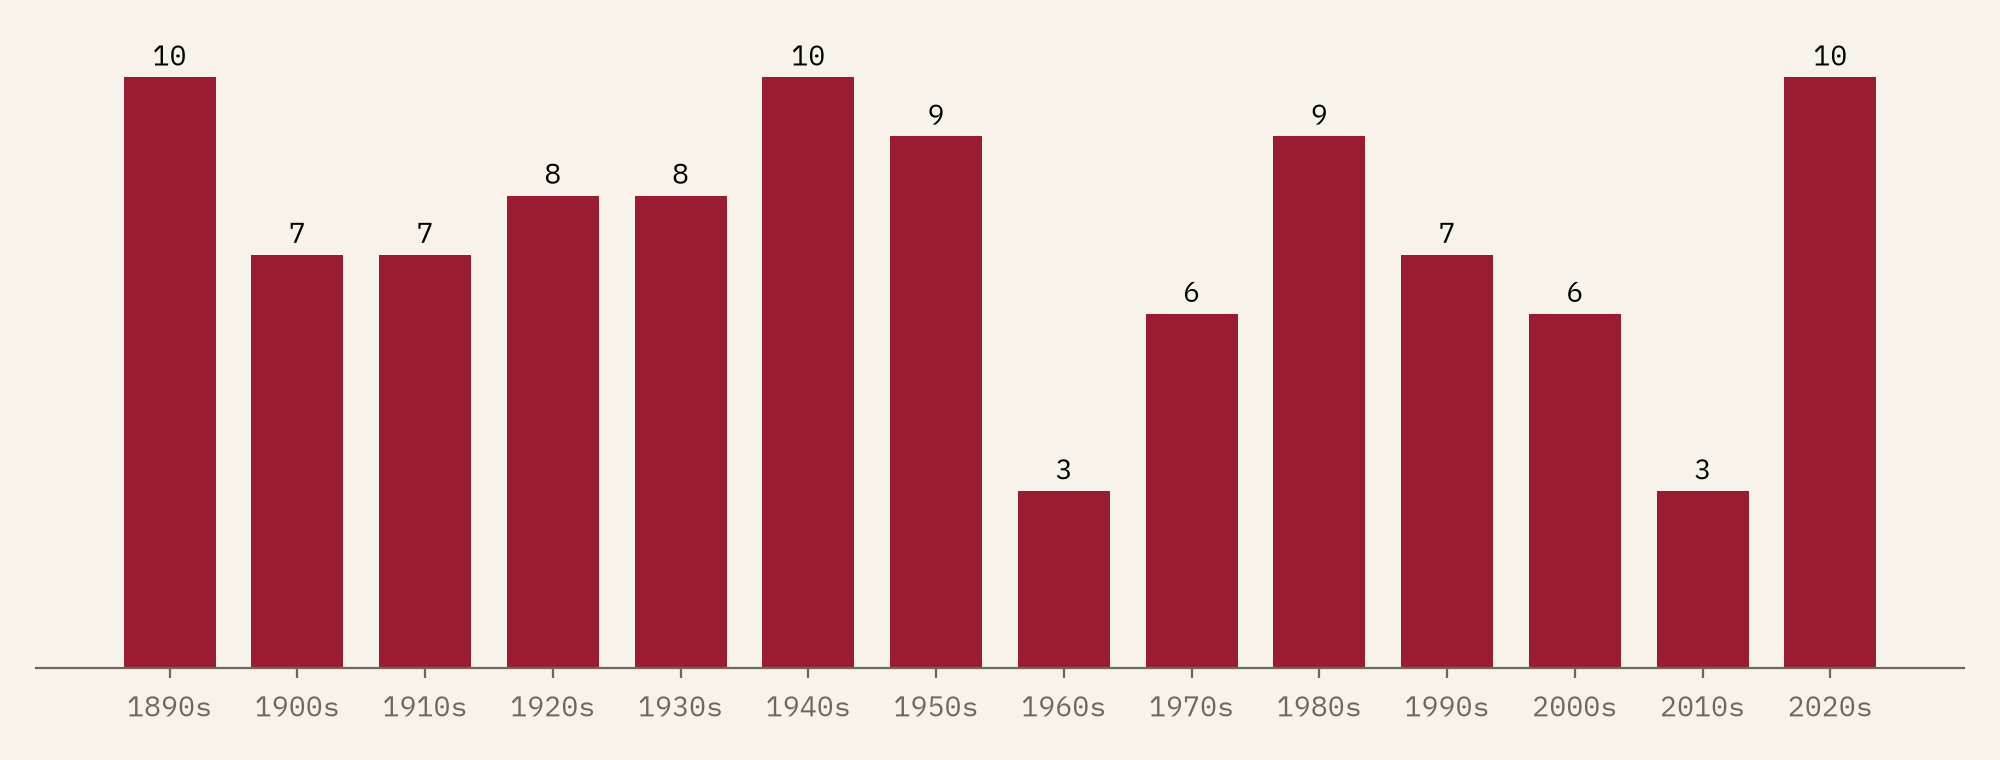
\includegraphics[width=.9\textwidth]{f_peaks.png}
\caption{Number of clubs (with twenty or more league seasons) whose best decade, by average league position, was each decade.}\label{fig:peaks}\end{figure}

\section{Discussion}
The map shows two geographies. One is the geography of founding: the league was made by the cotton towns of Lancashire and the industrial Midlands, and the North dominated the top flight until the 1930s. The other is the geography of population and money: London and the South, slow to take up professional football, filled the lower divisions after 1920 and the top flight increasingly after 1960. The North has kept its great city clubs, which still win most titles, but lost the middle: the towns of thirty to a hundred thousand people that supported top-flight or second-tier clubs before 1960. The crowd peak of the late 1940s was national, and so was the decline; the recovery since 1986 has been national too, which is why the lower divisions' crowds in 2024-25 are within reach of their post-war level.

\section{Limitations}
Crowd figures before about 1925 are estimates, often from newspaper reports, and the source's figures for all eras are compiled from several places; they should be read as orders of magnitude for early seasons and as good approximations later. Two recent seasons have no crowd data. Clubs are drawn at their present or last ground, not at every ground they used, so early London and Manchester positions are approximate (Woolwich Arsenal played in Plumstead until 1913). League position and crowd are only two measures of size: cup success, wealth, European football and fame are not here. Regions are present-day ONS regions applied to the whole period. The towns are a judgement about what each club represents.

\section{Conclusion}
English league football began as a northern and Midlands game, reached its biggest crowds in 1948-49, lost 60\% of them by 1985-86 and has won most back. Over the same years its centre moved south, its titles concentrated in a few great northern cities and London, and 39 towns lost their league club.

\section*{Data and code availability}
The interactive map is at \url{https://maps.tristanhotham.com/who-was-big-when/}. Code and derived data (per-club, per-season tables with average home league gates, per-season totals, club peaks, lost towns and all results) are at \url{https://github.com/Tristan-Hotham/who-was-big-when} and archived with this paper at \url{https://doi.org/10.5281/zenodo.23844507}. Match results are from engsoccerdata and openfootball; crowd figures are derived from englishfootballleaguetables.co.uk and credited to it. Derived data and text are released under CC BY 4.0, code under the MIT licence.

\section*{AI statement}
I wrote the text, with drafting and editing assistance from Claude (Anthropic), which also helped prepare the analysis code. I reviewed and checked all text and results.

\begin{thebibliography}{9}
\bibitem[Curley(2016)]{curley} Curley, J. P. (2016 and later) engsoccerdata: English soccer data. R package. \url{https://github.com/jalapic/engsoccerdata}. \url{https://doi.org/10.5281/zenodo.13158}
\bibitem[Dobson and Goddard(2011)]{dobson} Dobson, S. and Goddard, J. (2011) \emph{The Economics of Football}. 2nd edn. Cambridge: Cambridge University Press.
\bibitem[English Football League Tables(2026)]{eflt} English Football League Tables (2026) Average league gates, by season. \url{https://www.englishfootballleaguetables.co.uk/}
\bibitem[Office for National Statistics(2023)]{ons} Office for National Statistics (2023) Regions and counties boundaries. Open Government Licence v3.0.
\bibitem[openfootball(2026)]{openfootball} openfootball (2026) England: football.db match data. Public domain. \url{https://github.com/openfootball/england}
\bibitem[Russell(1997)]{russell} Russell, D. (1997) \emph{Football and the English: A Social History of Association Football in England, 1863 to 1995}. Preston: Carnegie.
\bibitem[Szymanski and Kuypers(1999)]{szymanski} Szymanski, S. and Kuypers, T. (1999) \emph{Winners and Losers: The Business Strategy of Football}. London: Viking.
\bibitem[Taylor(1990)]{taylor} Taylor, P. (1990) \emph{The Hillsborough Stadium Disaster: Final Report}. London: HMSO.
\end{thebibliography}
\end{document}
